\section{Methodology and Analysis}
\begin{frame}{}
  \Huge
  \centering
  \textbf{Methodology and Analysis}
  \normalsize
\end{frame}

\begin{frame}{Tools and Libraries Used}
  \small
  \begin{multicols}{3}
  \begin{itemize}
  \setlength\itemsep{-0.5em}
  \item Python 3.11.11
  \item Jupyter Notebook
  \item VS Code
  \item Kaggle for Fine-Tuning
  \item datasets
  \item pandas
  \item numpy
  \item faiss
  \item lightning
  \item torch
  \item torchvision
  \item tensorflow
  \item opencv-python
  \item opencv-python-headless
  \item albumentations
  \item PIL (Pillow)
  \item fashion-clip
  \item streamlit
  \item sqlalchemy
  \item psycopg2-binary
  \item alembic
  \item pydantic
  \item python-dotenv
  \item google-generativeai
  \item ipykernel
  \item scikit-learn
  \item tqdm
  \item requests
  \end{itemize}
  \end{multicols}
  \end{frame}


\begin{frame}{YOLOS Model}
  \small
  YOLOS (You Only Look One-level Series) is a Vision Transformer (ViT) trained using the DETR loss. Despite its simple design, a base-sized YOLOS model achieves an impressive \textbf{42 AP} (Average Precision) on the COCO 2017 validation dataset.
  \normalsize
  \vspace{0.5em}

  \textbf{YOLOS-Small Details:}
  \begin{itemize}
  \item Pre-trained for 200 epochs on ImageNet-1k.
  \item Fine-tuned for 150 epochs on COCO dataset.
  \item Achieves an AP of 36.1 on COCO 2017 validation.
\end{itemize}
\vspace{0.5em}
\small
We fine-tuned the YOLOS-Small model on the Fashionpedia dataset for object detection tasks. The model was trained using PyTorch Lightning’s Trainer class for 1 epoch.

\end{frame}

\begin{frame}{YOLOS Model Architecture}
\begin{figure}[H]
  \centering
  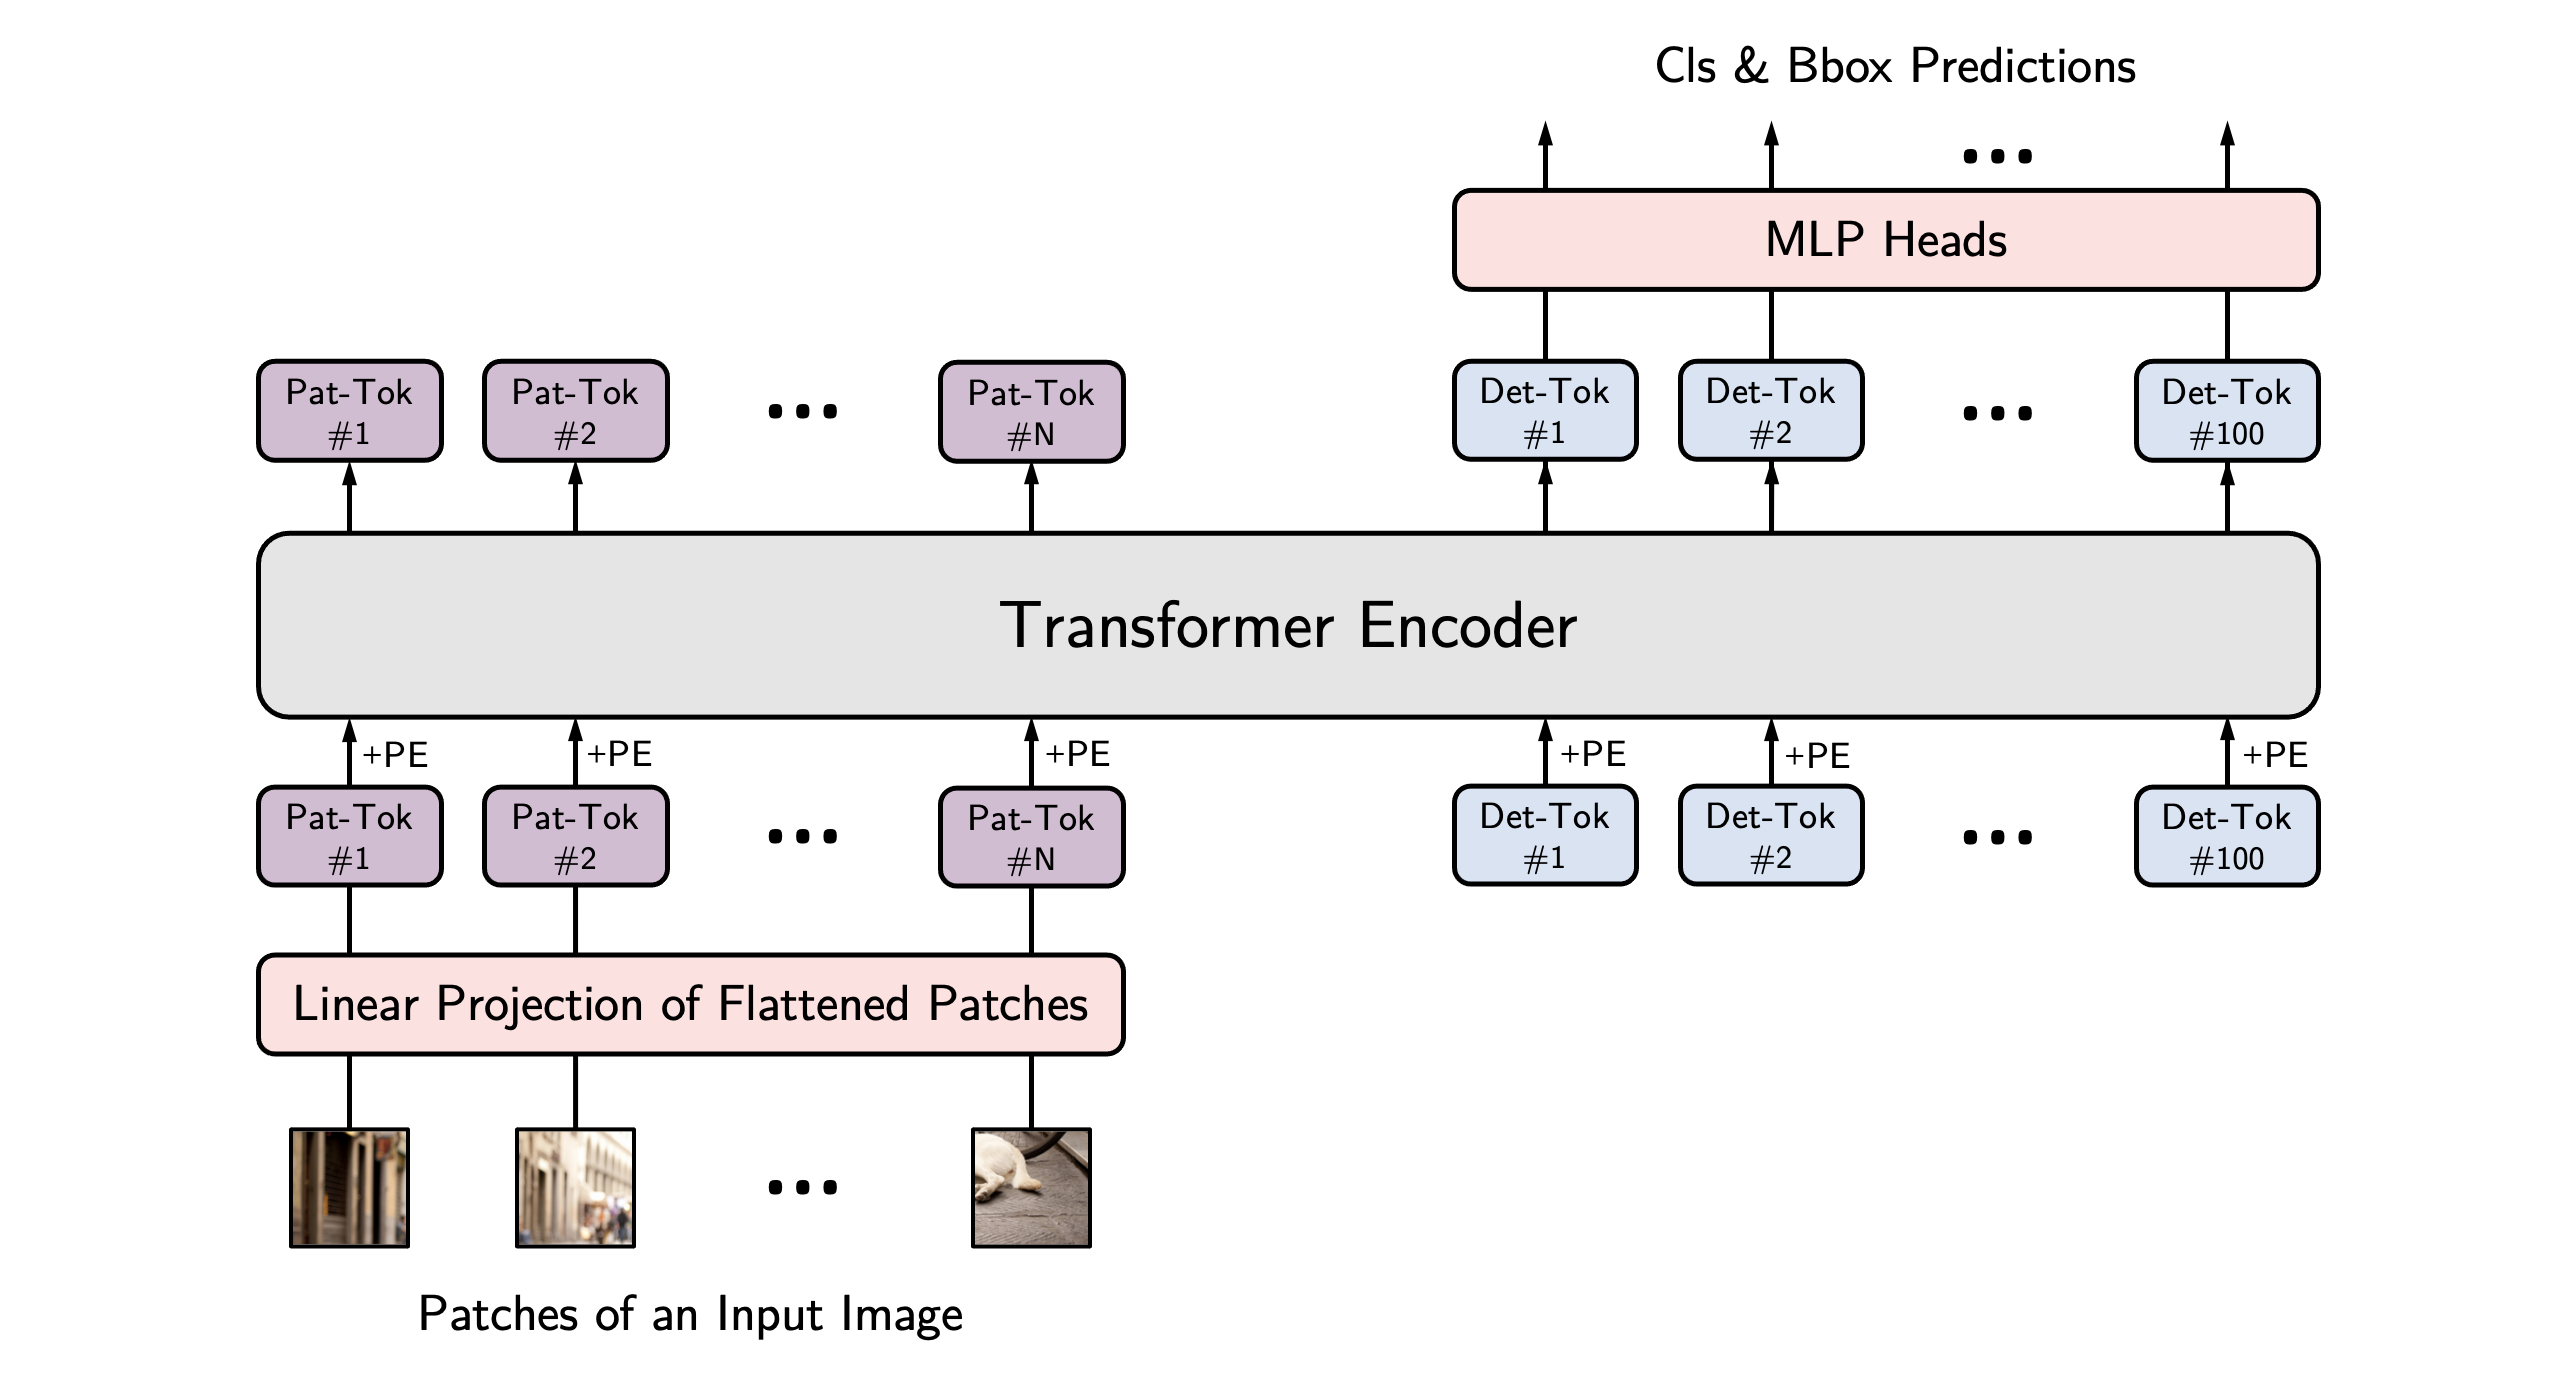
\includegraphics[width=0.85\textwidth]{images/yolos_architecture.png}
\end{figure}
\end{frame}

\begin{frame}{FashionCLIP Overview}
  \textbf{FashionCLIP} is a domain-specific adaptation of the original CLIP model, fine-tuned on a large corpus of fashion-related images and textual descriptions.

  \vspace{0.5em}

  It uses:
  \begin{itemize}
      \item \textbf{ViT-B/32 Transformer} as the image encoder.
      \item \textbf{Masked self-attention Transformer} as the text encoder.
  \end{itemize}

  Both encoders are trained jointly using a contrastive loss to maximize the similarity between corresponding (image, text) pairs.
  \end{frame}

  \begin{frame}{FashionCLIP Overview}

  \begin{figure}[H]
      \centering
      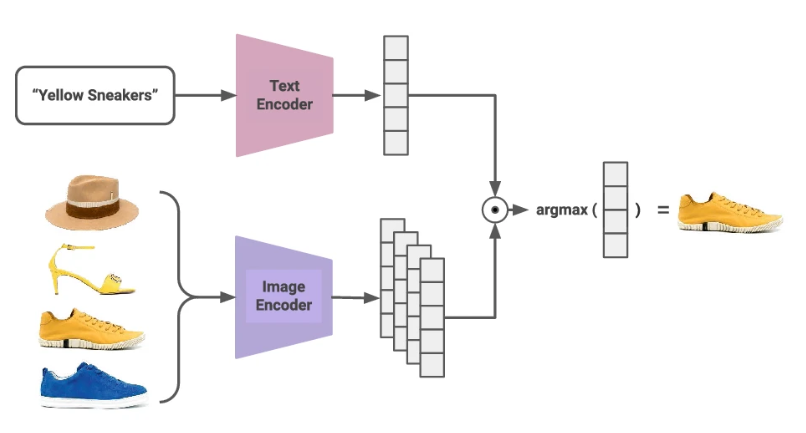
\includegraphics[width=0.8\textwidth]{images/fashion-clip.png}
  \end{figure}
  \end{frame}

  \begin{frame}{Shared Vector Space}
  FashionCLIP, like CLIP, creates a \textbf{shared vector space} for images and text.

  \vspace{0.5em}

  \begin{figure}[H]
      \centering
      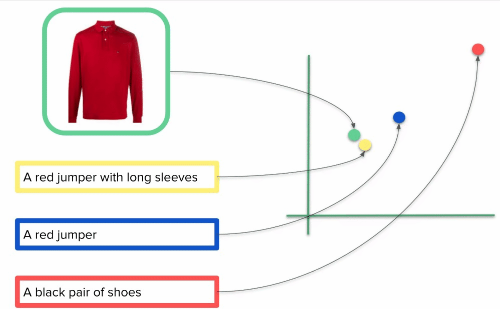
\includegraphics[width=0.5\textwidth]{../report_final/images/shared-vs.png}
  \end{figure}
  \end{frame}

  \begin{frame}{Image and Text Encoders}

  \begin{figure}[H]
      \centering
      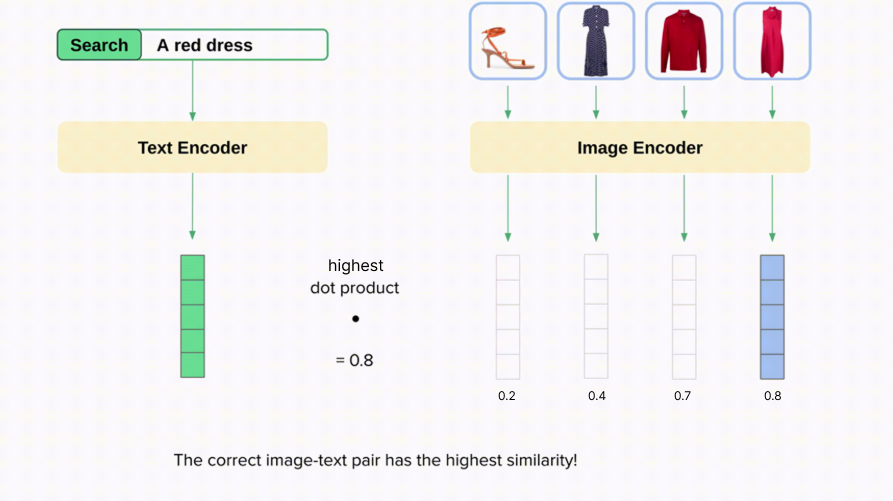
\includegraphics[width=0.8\textwidth]{../report_final/images/dotprod.png}
  \end{figure}
  \end{frame}

  \begin{frame}{Similarity Computation}
  The similarity between an image and a text embedding is computed using \textbf{cosine similarity}:

  \[
  \text{Similarity}(\mathbf{I}, \mathbf{T}) = \frac{\mathbf{I} \cdot \mathbf{T}}{\|\mathbf{I}\| \|\mathbf{T}\|}
  \]
\small
  Where:
  \begin{itemize}
      \setlength\itemsep{-0.25em}
      \item $\mathbf{I}$ = Image embedding vector
      \item $\mathbf{T}$ = Text embedding vector
      \item $\cdot$ = Dot product
      \item $\|\mathbf{I}\|, \|\mathbf{T}\|$ = Vector norms (magnitudes)
  \end{itemize}
  \end{frame}

  \begin{frame}{Usage in Our Project}
  In our system:
  \begin{itemize}
      \item FashionCLIP generates embeddings for \textbf{inventory images} and \textbf{textual descriptions}.
      \item These embeddings are stored in a \textbf{FAISS database} for fast similarity search.
  \end{itemize}

  \vspace{0.5em}

  At query time:
  \begin{itemize}
      \item User inputs an \textbf{image} (e.g., a cropped garment detected by YOLOS) or \textbf{text} (e.g., "red summer dress").
      \item FashionCLIP embeds the query.
      \item Closest matches from the inventory are retrieved based on cosine similarity.
  \end{itemize}
  \end{frame}

  \begin{frame}{Evaluation Metric: Recall@6}
    \small
    For text-based retrieval, we evaluated the model using the \textbf{Recall@K} metric, which measures the proportion of relevant items retrieved in the top-K results.

    \vspace{0.5em}

    Given:
    \begin{itemize}
        \setlength\itemsep{-0.25em}
        \item \( T = \{ t_1, t_2, \ldots, t_n \} \) : Text embeddings
        \item \( I = \{ i_1, i_2, \ldots, i_n \} \) : Image embeddings
        \item Similarity: \( s(t_k, i_j) = t_k^\top i_j \)
    \end{itemize}
    \normalsize
    \[
    \text{correct} = \sum_{k=1}^{n} \mathbf{1}\{k \in \text{Top}_5(t_k)\}
    \quad \quad
    \text{Recall} = \frac{\text{correct}}{n}
    \]
    \small
    \vspace{0.5em}

    We used \textbf{Recall@6} for evaluation and achieved a score of \textbf{0.68}, indicating that 68\% of the time, the relevant item is found in the top 5 results.
    \end{frame}

\begin{frame}{}
  \Huge
  \centering
  \textbf{Demo}
  \normalsize
\end{frame}
